\section{\texorpdfstring{TIM2 - čítač}{TIM2 - citac}}

% =====================================================================================================================
	\begin{frame}
    \frametitle{TIM2 - čítač pro obecné použití}
		
		\begin{center}
			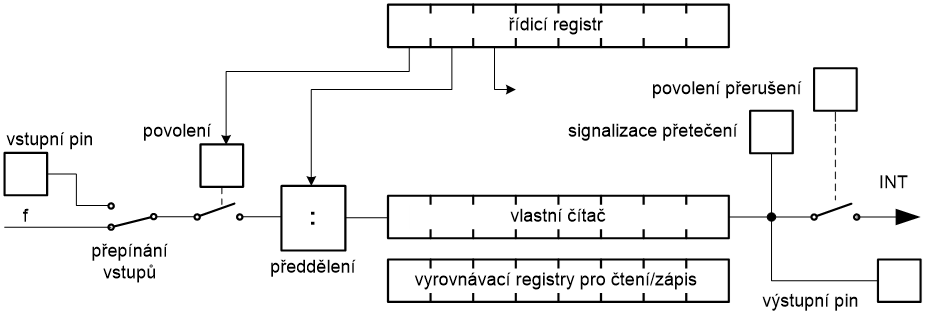
\includegraphics[width=0.7\textwidth]{fig/tim2_block_diag.png}
		\end{center}

		\textbf{Základní parametry}
		\small
		\begin{itemize}
			\item Šířka 16 bit s 4 bit před-děličkou hodinového signálu,
			\item režimy:
			\begin{itemize}
				\item zachycení vstupu (Input Capture),
				\item porovnání výstupu (Output Compare),
				\item PWM.
			\end{itemize}
			\item možnost generovat přerušení pro ve všech režimech a přetečení.
		\end{itemize}
		
	\end{frame}
	
% =====================================================================================================================
	\begin{frame}
    \frametitle{TIM2 - čítání}
		
		\begin{center}
			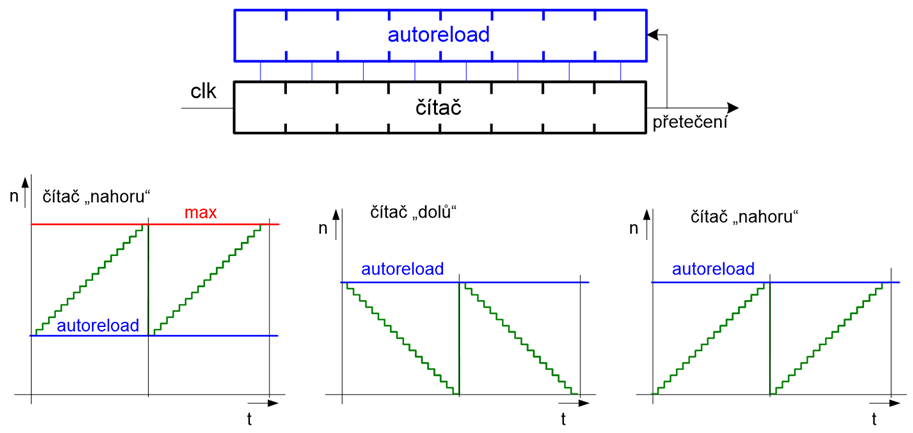
\includegraphics[width=0.9\textwidth]{fig/tim2_counting.png}
		\end{center}

		\begin{itemize}
			\item Obvykle lze čítat jak nahoru do nastavené hodnoty (TIM1) tak
			\item dolů z přednastavené hodnoty (TIM1),
			\item konkrétně TIM2 čítá jen nahoru.
		\end{itemize}
		
	\end{frame}
	
% =====================================================================================================================
	\begin{frame}
    \frametitle{TIM2 - Input Capture}
		
		\begin{center}
			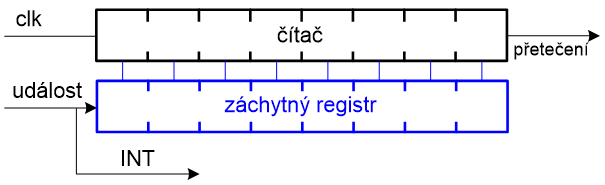
\includegraphics[width=0.6\textwidth]{fig/tim2_capture.png}
		\end{center}

		\begin{itemize}
			\item Sleduje se konkrétní událost, například změna stavu (hrana) některého vstupu,
			\item v okamžiku výskytu události se zachytí stav čítače do záchytného registru,
			\item lze žádat o akci prostřednictvím přerušení,
			\item umožňuje přesný záznam času události.
		\end{itemize}
		
	\end{frame}
	
% =====================================================================================================================
	\begin{frame}
    \frametitle{TIM2 - Output Compare}
		
		\begin{center}
			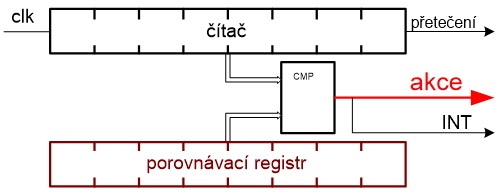
\includegraphics[width=0.6\textwidth]{fig/tim2_compare.png}
		\end{center}

		\begin{itemize}
			\item Porovnává se aktuální hodnota čítače s referenční hodnotou v registru,
			\item v okamžiku shody se provede definovaná akce, například dojde k přenastavení určitého digitálního výstupu,
			\item lze žádat o akci prostřednictvím přerušení,
			\item umožňuje provést časově závislou akci bez zatížení programu.
		\end{itemize}
		
	\end{frame}
	
% =====================================================================================================================
	\begin{frame}
    \frametitle{TIM2 - PWM}
		
		\begin{center}
			\includegraphics[width=0.9\textwidth]{fig/tim2_PWM.png}
		\end{center}

		\begin{itemize}
			\item ve své podstatě jde o rozšíření funkce Compare,
			\item puls je vystaven na shodu hodnoty a smazán na přetečení čítače,
			\item takto generovaná PWM zarovnaná vůči jedné hraně (zde doběžná hrana).
		\end{itemize}
		
	\end{frame}
	
% =====================================================================================================================
	\begin{frame}
    \frametitle{Návod v materiálech na cvičení}

		\begin{center}
			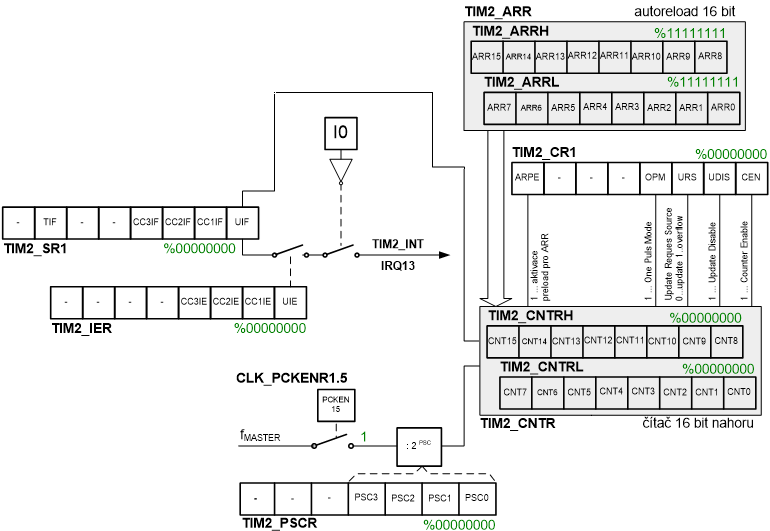
\includegraphics[width=0.80\textwidth]{fig/tim2_navod.png}
		\end{center}
		
	\end{frame}
	
% =====================================================================================================================
	\begin{frame}
    \frametitle{Význam registru TIM2\_CR1}

		\textbf{C}ontrol \textbf{R}egister 1

		\begin{center}
			\tiny
			\begin{tabular}{| p{9mm} | p{9mm} | p{9mm} | p{9mm} | p{9mm} | p{9mm} | p{9mm} | p{9mm} |}
				\hline
				\hline
				\textbf{ARPE} & \textbf{-} & \textbf{-} & \textbf{-} & \textbf{OPM} & \textbf{URS} & \textbf{UDIS} & \textbf{CEN} \\
				\hline
				\hline
			\end{tabular}
		\end{center}
				
		\begin{itemize}
			\item slouží pro nastavení chování čítače během čítání,
			\item stav po resetu 0x00,
			\small
			\begin{center}
				\begin{tabular}{l p{80mm}}
					\textbf{ARPE} & Povolení update hodnoty ARR registru pomocí stínového registru. \\
					\textbf{OPM} & Povolení zastavení čítače při update hodnoty z ARR registru. \\
					\textbf{URS} & Výběr zdroje přerušení UI podle 0:update nebo podle 1:přetečení.  \\
					\textbf{UDIS} & Disable pro update. \\
					\textbf{CEN} & Povolení čítání.
				\end{tabular}
			\end{center}
		\end{itemize}
		
	\end{frame}
	
% =====================================================================================================================
	\begin{frame}
    \frametitle{Význam registru TIM2\_IER}

		\textbf{I}nterrupt \textbf{E}nable \textbf{R}egister

		\begin{center}
			\tiny
			\begin{tabular}{| p{9mm} | p{9mm} | p{9mm} | p{9mm} | p{9mm} | p{9mm} | p{9mm} | p{9mm} |}
				\hline
				\hline
				\textbf{-} & \textbf{-} & \textbf{-} & \textbf{-} & \textbf{CC3IE} & \textbf{CC2IE} & \textbf{CC1IE} & \textbf{UIE} \\
				\hline
				\hline
			\end{tabular}
		\end{center}
				
		\begin{itemize}
			\item slouží pro povolení jednotlivých zdrojů přerušení,
			\item stav po resetu 0x00,
			\small
			\begin{center}
				\begin{tabular}{l p{80mm}}
					\textbf{CC3IE} & Povolení přerušení capture compare kanál 3. \\
					\textbf{CC3IE} & Povolení přerušení capture compare kanál 2.  \\
					\textbf{CC3IE} & Povolení přerušení capture compare kanál 1. \\
					\textbf{UIE} & Povolení přerušení při update nebo přetečení (podle URS bitu, viz předchozí slide).
				\end{tabular}
			\end{center}
		\end{itemize}
		
	\end{frame}
	
% =====================================================================================================================
	\begin{frame}
    \frametitle{Význam registru TIM2\_SR1}

		\textbf{S}tatus \textbf{R}egister 1

		\begin{center}
			\tiny
			\begin{tabular}{| p{9mm} | p{9mm} | p{9mm} | p{9mm} | p{9mm} | p{9mm} | p{9mm} | p{9mm} |}
				\hline
				\hline
				\textbf{-} & \textbf{-} & \textbf{-} & \textbf{-} & \textbf{CC3IF} & \textbf{CC2IF} & \textbf{CC1IF} & \textbf{UIF} \\
				\hline
				\hline
			\end{tabular}
		\end{center}
				
		\begin{itemize}
			\item slouží pro signalizaci, že došlo k některé události - vlajky,
			\item stav po resetu 0x00,
			\small
			\begin{center}
				\begin{tabular}{l p{80mm}}
					\textbf{CC3IF} & Vlajka přerušení capture compare kanál 3. \\
					\textbf{CC3IF} & Vlajka přerušení capture compare kanál 2.  \\
					\textbf{CC3IF} & Vlajka přerušení capture compare kanál 1. \\
					\textbf{UIE} & Vlajka přerušení při update nebo přetečení (podle URS bitu, viz předchozí slide).
				\end{tabular}
			\end{center}
		\end{itemize}
		
	\end{frame}
	
% =====================================================================================================================
	\begin{frame}
    \frametitle{Význam registru TIM2\_PSCR}

		\textbf{P}re\textbf{sc}aler \textbf{R}egister

		\begin{center}
			\tiny
			\begin{tabular}{| p{9mm} | p{9mm} | p{9mm} | p{9mm} | p{9mm} | p{9mm} | p{9mm} | p{9mm} |}
				\hline
				\hline
				\textbf{-} & \textbf{-} & \textbf{-} & \textbf{-} & \textbf{PSC3} & \textbf{PSC2} & \textbf{PSC1} & \textbf{PSC0} \\
				\hline
				\hline
			\end{tabular}
		\end{center}
				
		\begin{itemize}
			\item slouží pro nastavení předděličky pro vstupní hodinový signál čítače,
			\item stav po resetu 0x00,
			\small
			\begin{center}
				\begin{tabular}{l p{80mm}}
					\textbf{PSC3:0} & Exponent základu 2, výsledná hodnota udává předdělící poměr. \\
				\end{tabular}
			\end{center}
		\end{itemize}
		
		Dělící poměr:
		\begin{center}
			$D = 2^{PSC}$
		\end{center}
		
		
		\begin{itemize}
			\item Získáváme hodnotu mezi \textbf{1} a \textbf{32768}.
		\end{itemize}
		
	\end{frame}

% =====================================================================================================================
	\begin{frame}
    \frametitle{Program čekání pomocí TIM2}
		
		Pomocí čítače TIM2 realizujte časování programu:
		\begin{enumerate}
			\item čekání na přetečení čítače,
			\item změna výstupu jeho negací,
			\item skok na bod 1.
		\end{enumerate}
		
	\end{frame}
	
% =====================================================================================================================
	\begin{frame}
    \frametitle{Program čekání pomocí TIM2 - definiční konstanty}
		
		\begin{center}
			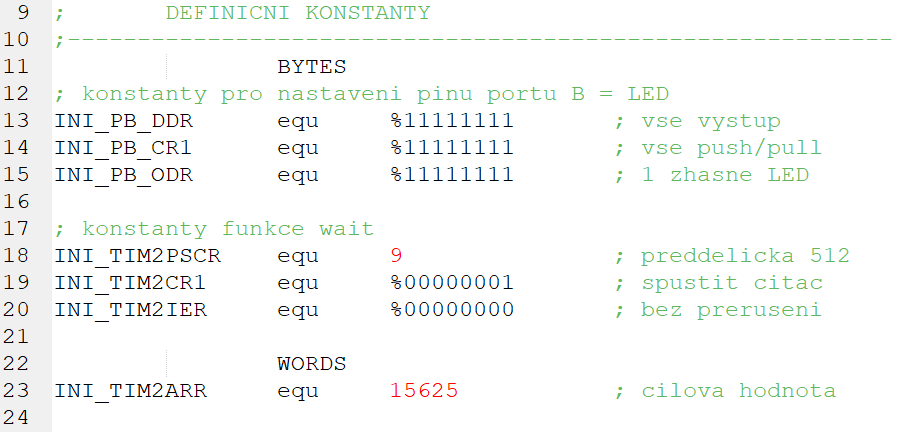
\includegraphics[width=0.80\textwidth]{fig/prg_tim2_define.png}
		\end{center}
		
	\end{frame}
	
% =====================================================================================================================
	\begin{frame}
    \frametitle{Program čekání pomocí TIM2 - smyčka}
		
		\begin{center}
			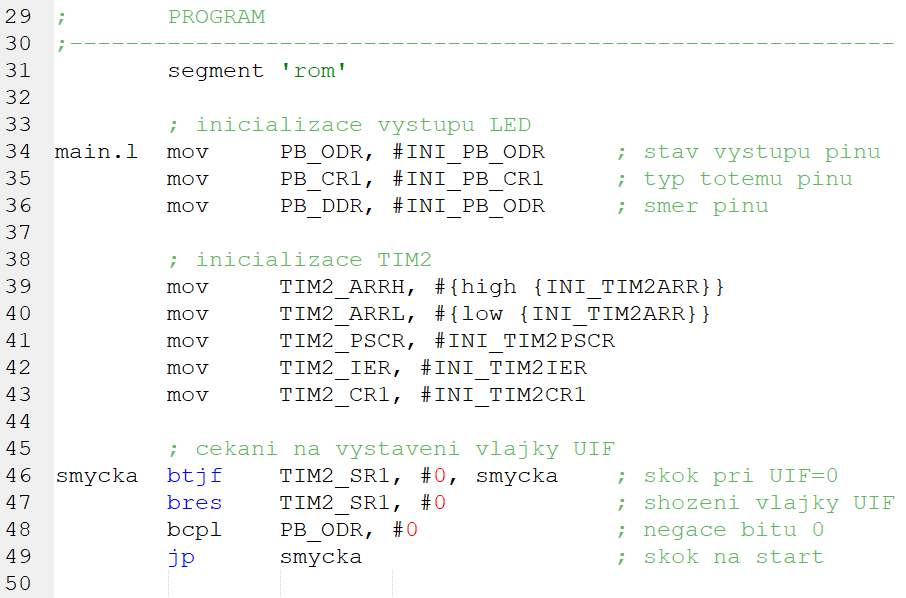
\includegraphics[width=0.80\textwidth]{fig/prg_tim2_loop.png}
		\end{center}
		
	\end{frame}